% !TEX root = ../report.tex
\chapter{Evaluation}
In this chapter it will be described how the proposed approaches were compared against the standard implementation and how they were evaluated.\\
At first the data sets used for the comparison and the evaluation are described, then the \acf{ROS} setup will be explained and in the last section, the evaluation procedure itself will be described.

\section{Data sets}
Both of the used data sets were captured in a room equipped with a motion tracking system, VICON, which provided the ground truth for the comparison and the evaluation. As the whole setup is based on \ac{ROS}, the data sets were recorded with rosbags. The rosbags contain at least the following topics:
\begin{itemize}
  \item The grayscale images as sensor\_msgs.msg.Image in the topic /cam0/image\_raw
  \item The ground truth as geometry\_msgs.msg.PointStamped in the topic /camera\_imu/vrpn\_client/estimated\_transform respective
\end{itemize}

The recorded rosbags were afterwards splitted into parts which do not contain any loop closure as loop closures would prohibit a fair comparison between the standard and the proposed new map merging approach.

For the evaluation each client took the data from a seperate splitted rosbag simulating two clients running the same time in the same area.

\subsection{Hand held}
The hand held data set (vi\_loops\_close and vi\_loosp\_far) was recorded with a camera rig walking loops while facing the wall. In the data set ``vi\_loops\_close'', a frame of it shown in \autoref{fig:dataset_close}, the camera was close to the wall. In the data set ``vi\_loops\_far'', a frame of it shown in \autoref{fig:dataset_far}, the camera was far from the wall.

\begin{figure}[H]
  \centering
  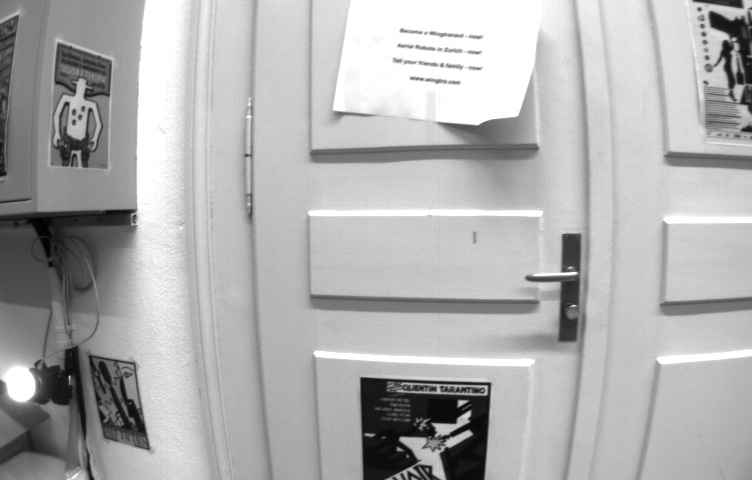
\includegraphics[width=0.75\textwidth]{images/frame0000}
  \caption{Frame from the hand held data set close to the wall}
  \label{fig:dataset_close}
\end{figure}

\begin{figure}[H]
  \centering
  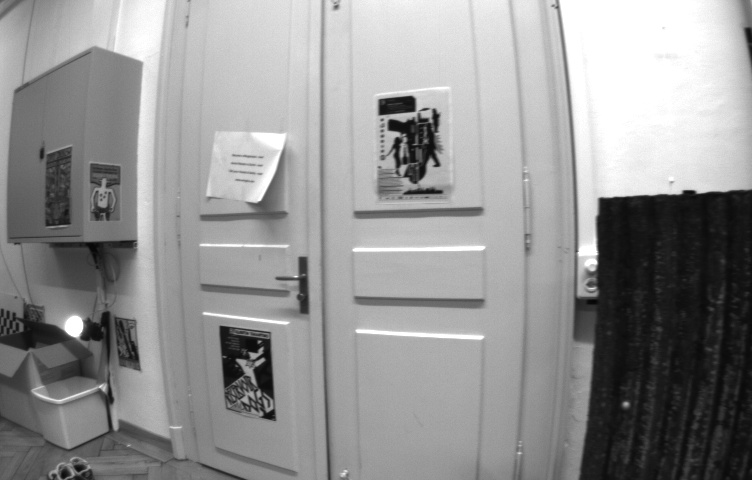
\includegraphics[width=0.75\textwidth]{images/frame0014}
  \caption{Frame from the hand held data set far from the wall}
  \label{fig:dataset_far}
\end{figure}

\subsection{\acf{UAV}}
The \ac{UAV} used to record this data set (vi\_loops\_uav) is shown in \autoref{fig:uav}. In this data set loops were flown while the camera of the \ac{UAV} was facing the wall. A frame of the recorded data set is shown in \autoref{fig:dataset_uav}.

\begin{figure}[H]
  \centering
  \includegraphics[width=0.75\textwidth]{images/uav}
  \caption{The used \ac{UAV}}
  \label{fig:uav}
\end{figure}

\begin{figure}[H]
  \centering
  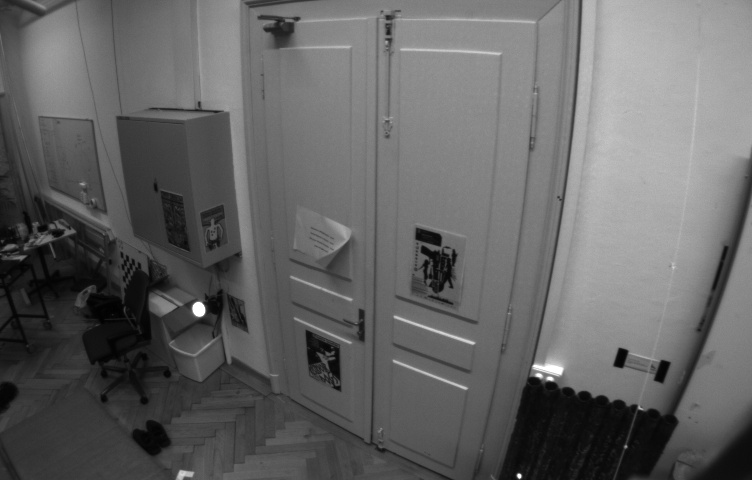
\includegraphics[width=0.75\textwidth]{images/frame0128}
  \caption{Frame from the \ac{UAV} data set}
  \label{fig:dataset_uav}
\end{figure}

\section{\acf{ROS} setup}
As already mentioned, the data set for the two clients were created by splitting a bigger data set recorded with only one client. Because the splitted data sets don't have the same timing, a retiming \ac{ROS} node, explained in the next subsection, was written to work around this issue.\\
To get the ground truth in a usable format, a record \ac{ROS} node, explained in \autoref{subsec:record_node}, was written which receives the ground truth position from the retimin \ac{ROS} node and writes it into a text file.\\

The whole \ac{ROS} setup is illustrated in \autoref{fig:ros_setup}.

\tikzstyle{block} = [draw, fill=white, rectangle, minimum height=3em, minimum width=6em]
\tikzstyle{point} = [coordinate]
\begin{figure}[H]
  \centering
  \begin{tikzpicture}[auto, node distance=2cm,>=latex']
		\node [block] (client_1) {rosbag for client 1};
		\node [point] (p1) [right= 1.0cm of client_1]{};
		\node [point] (p2) [below= 0.55cm of p1]{};
		
		\node [block] (client_2) [below = 1.5cm of client_1.west, anchor=west] {rosbag for client 2};	
		\node [point] (p3) [right = 1.0cm of client_2]{};
		\node [point] (p4) [above = 0.5cm of p3]{};
		
		\node [block] (retiming) [below right =-0.3cm and 2cm of client_1] {retiming node};
    \node [point] (p5) [right = 1cm of retiming, yshift=0.2cm]{};
    \node [point] (p7) [above = 0.9cm of p5]{};
    \node [point] (p6) [right = 1cm of retiming, yshift=-0.2cm]{};
    \node [point] (p8) [below = 0.9cm of p6]{};

    \node [block] (slam) [above right = 0.001cm and 2cm of retiming] {SLAM System};
    \node [block] (recording) [below right = 0.001cm and 2cm of retiming] {recording node};
		
		%\draw [-] (publish_image) -- node[name=u] {/cam0/image\_raw, /camera\_imu/vrpn\_client/estimated\_transform} (p1);
		%\draw [-] (publish_image) -- node[name=u] {grayscale images, ground truth positions} (p1);
		\draw [-] (client_1) -- node[name=u] {} (p1);
		\draw [-] (p1) -- (p2);
		\draw [-] (p3) -- (p4);
		
		\draw [-] (client_2) -- (p3);
		
		\draw [->] (p2) -- (p2-|retiming.west);
		\draw [->] (p4) -- (p4-|retiming.west);

    \draw [-] ([yshift=0.2cm]retiming.east) -- (p5);
    \draw [-] ([yshift=-0.2cm]retiming.east) -- (p6);

    \draw [-] (p5) -- (p7);
    \draw [-] (p6) -- (p8);

    \draw [->] (p7) -- (p7-|slam.west);
    \draw [->] (p8) -- (p8-|recording.west);
	\end{tikzpicture}
  \caption{\ac{ROS} setup}
  \label{fig:ros_setup}
\end{figure}

\subsection{Re-timing node}
The re-timing \ac{ROS} node subscribes to the topics providing the ground truth position and the grayscale image and republishes the messages of these topics with the time stamp set to the current system time.

\subsection{Recording node}
\label{subsec:record_node}
The recording \ac{ROS} node subscribes to the topic, the re-timing \ac{ROS} node publishes, which contains the ground truth position. It saves the ground truth positions into a list and at the end writes all the positions together with their time stamps into a text file.

\section{Evaluation}
